\documentclass{report}
% Change "article" to "report" to get rid of page number on title page
\usepackage{amsmath,amsfonts,amsthm,amssymb}
\usepackage{setspace}
\usepackage{Tabbing}
\usepackage{fancyhdr}
\usepackage{lastpage}
\usepackage{extramarks}
\usepackage{chngpage}
\usepackage{soul,color}
\usepackage{listings}
\usepackage{enumerate}
\usepackage{graphicx,float,wrapfig}
\usepackage{pifont}
\usepackage{graphicx}
\usepackage[english]{babel}
\usepackage{tikz}
\usepackage[]{algorithm2e}
% In case you need to adjust margins:
\topmargin=-0.45in      %
\evensidemargin=0in     %
\oddsidemargin=0in      %
\textwidth=6.5in        %
\textheight=9.0in       %
\headsep=0.25in         %

\title{Assignment 2 - Comp 632 - Machine Learning}

% Homework Specific Information
\newcommand{\hmwkTitle}{Assignment 2}                     % Adjust this
\newcommand{\hmwkDueDate}{Wednesday, February 18 2015}                           % Adjust this
\newcommand{\hmwkClass}{COMP 632}


\newcommand{\hmwkClassInstructor}{Dr. Doina Precup}
\newcommand{\hmwkAuthorName}{Geoffrey Stanley}
\newcommand{\hmwkAuthorNumber}{260645907}
\newcommand{\Pp}{\mathbb{P}}
\newcommand{\Ev}{\mathbb{E}}
\newcommand{\cov}{\text{Cov}}
\newcommand{\Z}{\mathbb{Z}}
\newcommand{\R}{\mathbb{R}}
\newcommand{\dd}{\, \mathrm{d}}

% Setup the header and footer
\pagestyle{fancy}                                                       %
\lhead{\hmwkAuthorName}                              %
\chead{}
\rhead{\hmwkClass: \hmwkTitle}                                          %

\lfoot{}
\cfoot{}                                                                %
\rfoot{Page\ \thepage\ of\ \pageref{LastPage}}                          %
\renewcommand\headrulewidth{0.4pt}                                      %
\renewcommand\footrulewidth{0.4pt}                                      %

% This is used to trace down (pin point) problems
% in latexing a document:
%\tracingall
\definecolor{mygreen}{rgb}{0,0.6,0}
\lstset{commentstyle=\color{mygreen}, frame=single,  language=R, showspaces=false, showstringspaces=false}

%%%%%%%%%%%%%%%%%%%%%%%%%%%%%%%%%%%%%%%%%%%%%%%%%%%%%%%%%%%%%
% Make title
\title{\vspace{2in}\textmd{\textbf{\hmwkClass:\ \hmwkTitle}}\\
\normalsize\vspace{0.1in}\small{Due\ on\ \hmwkDueDate}\\
\vspace{0.1in}\large{\textit{Presented to \hmwkClassInstructor}}\vspace{3in}}
\date{}
\author{\textbf{\hmwkAuthorName}\\
    \textbf{Student ID: \hmwkAuthorNumber}}
%%%%%%%%%%%%%%%%%%%%%%%%%%%%%%%%%%%%%%%%%%%%%%%%%%%%%%%%%%%%%

\begin{document}
\maketitle
\section*{Question 1}
\subsection*{A)}
For a function to be considered a kernel function the kernel matrix defined as
$K_{ij}=K(x_i,x_j)$ must have two properties:
\begin{enumerate}
  \item be symmetric
  \item be positive semidefinite
\end{enumerate}
As such, a Kernel matrix must abide by the following:
\begin{equation}
  K_{ij} = K_{ji}
\end{equation}
\begin{equation}
  z^{T}Kz\geq 0
\end{equation}
Where $z$ is an arbitrary vector. \\

A kernel function is also one that can be expressed as a dot product of the feature
vectors of the instances:
\begin{equation}
  K(x,z) = \phi (x) \cdot \phi (x)
\end{equation}
where $\phi$ is a feature maping of input features to a vector space. Further more,
as described by Bishop(2006) p.296 a kernel function can be a construction of kernel
functions such that
\begin{equation}
  k(x,z) = k_1(x,z) + k_2(x,z)
\end{equation}
In this particular case it would be usefull to decompose our $K_l$ kernal function
into:
\begin{equation}
  k_l(x,z) = k_1(x,z) + k_2(x,z) + ... + k_l(x,z)
\end{equation}
where the components of the decomposition evaluate the similarity of a particular
character length such that $k_1('ar','ark')=1$ and $k_2('ar','ark')=2$. Now, in order
to show that $K_l$ is a kernal function, we are left with having to create a feature
mapping onto some vector where dot products of those vector would result in the
similarity required.

For simplicity let's define our alphabet as being ${a,b,c}$
and our mapping to be onto a three dimensional vector representing our alphabet.
Now we can map an input string such as "ab" onto a vector $x=[1,1,0]$. Given another
string "bc" we can create $y=[0,1,1]$ where $x^Ty=1$. Expanding this mapping into
longer character combinations we can now define our vector space as being all combination
of character sequences of length 1 through $l$.

We now have multiple functions that can
be expressed in terms of a dot product of vectors whose sum is equal to our original $K_l$
function and have thus demonstrated that it is a kernal function.

\subsection*{B)}
As $l$ increases words will have a tendency of having higher scores when compared
with itself then any other words. This will result in a diagonal matrix.
\subsection*{C)}
Yes.
\subsection*{D)}

\section*{Question 2}
\subsection*{A)}
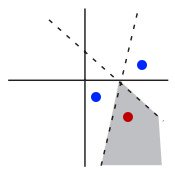
\includegraphics[width=175px, keepaspectratio]{3points.jpg}
\subsection*{B)}
The VC-dimension of this hypthesis class is 4. This is because it can successfully
shatter all configurations of 4 points. However, it would not be able to do so for all
configuration of 5 points.
\subsection*{C)}
The VC-dimension of any type of boolean combination of 2 linear classifiers is
also 4.

\section*{Question 3}
\subsection*{A)}
Given the log-likelihood of a hypothesis $h$ :

\begin{equation}
  \log L(h) = \sum_{i=1}^{m} \log P(y_i|x_i,h)
\end{equation}

And the probability of an example x belonging to class K as being :

\begin{equation}
  P(K | x) = 1 - \sum_{i=1}^{K-1}h^i(x)
\end{equation}

We can derive the log likelihood for a set of hypotheses and a given data set D as:

\begin{equation}
  \log L(h) = \sum_{i=1}^{m} \sum_{j=1}^{K} \log \left( 1 - \sum_{l=1}^{K-1}h^l(x_i) \right)
\end{equation}


\subsection*{B)}
\subsection*{C)}

\section*{Question 4}
\subsection*{A)}
\begin{center}
\begin{table}[h]
 \begin{tabular}{l|c|c|c|c|c|}
 \cline{2-6}
     & \multicolumn{5}{c|}{Folds}      \\ \cline{2-6}
     &  1  &  2  &  3  &  4  &  5 \\ \hline
\multicolumn{1}{|l|}{log L Train} & -2.103 & -2.077 & -2.031 & -1.979 & -2.033  \\ \hline
\multicolumn{1}{|l|}{log L Test} & -2.064 & -2.090 & -2.016 & -1.885 & -2.129  \\ \hline
\multicolumn{1}{|l|}{Training Accuracy} & 0.81\% & 0.81\% & 0.83\% & 0.81\% & 0.80\% \\ \hline
\multicolumn{1}{|l|}{Testing Accuracy} & 0.69\% & 0.69\% & 0.72\% & 0.87\% & 0.71\% \\ \hline
\end{tabular}
\end{table}
\end{center}
\subsection*{B)}
\subsection*{C)}
\begin{center}
\begin{table}[h]
 \begin{tabular}{l|l|l|l|l|l|l|l|l|l|l|}
 \cline{2-11}
     & \multicolumn{10}{c|}{Folds}      \\ \cline{2-11}
     & \multicolumn{2}{c|}{1} & \multicolumn{2}{c|}{2} & \multicolumn{2}{c|}{3} & \multicolumn{2}{c|}{4} & \multicolumn{2}{c|}{5} \\ \hline
\multicolumn{1}{|c|}{log L Train} & -0.231 & -1.428 & -0.174 & -1.435 & -0.222 & -1.560 & -0.253 & -1.434 & -0.223 & -1.371 \\ \hline
\multicolumn{1}{|c|}{log L Test} & -0.410 & -1.418 & -0.497 & -1.627 & -0.547 & -1.701 & -0.549 & -1.807 & -0.456 & -1.664 \\ \hline
\multicolumn{1}{|l|}{Training Accuracy} & \multicolumn{2}{c|}{0.82\%} & \multicolumn{2}{c|}{0.84\%} & \multicolumn{2}{c|}{0.83\%} & \multicolumn{2}{c|}{0.81\%} & \multicolumn{2}{c|}{0.83\%} \\ \hline
\multicolumn{1}{|l|}{Testing Accuracy} & \multicolumn{2}{c|}{0.72\%} & \multicolumn{2}{c|}{0.67\%} & \multicolumn{2}{c|}{0.69\%} & \multicolumn{2}{c|}{0.85\%} & \multicolumn{2}{c|}{0.74\%} \\ \hline
\end{tabular}
\end{table}
\end{center}
\subsection*{D)}
\subsection*{E)}

\end{document}
